

\chapter{\textit{Neural Ringer}: Alternativa de \textit{Trigger}}
\label{cap:metodologia}
\glsresetall

Em problemas de filtragem \textit{online} onde diferentes níveis de \textit{trigger} implementados de forma hierárquica, do sistema mais simples
ao mais robusto, é sempre atraente otimizar os primeiros níveis dessa cadeia. Uma vez que, ao se aumentar a eficiência de detecção
e a rejeição a eventos não interessantes para o estudo, diminui-se o número de vezes em que os sistemas de filtragem superiores,
muitas vezes de maior latência, sejam utilizados com eventos que claramente não são necessários para o estudo de interesse.

Em outras palavras é desejado que eventos que seriam eliminados em sistemas de filtragem mais complexos como os níveis 
hierárquicos superiores sejam eliminados pelos níveis inferiores. Assim, esses sistemas mais complexos somente se encarregariam
de eventos que sejam realmente necessário a utilização de algoritmos e ferramentas mais complexas para efetuar sua discriminação.

O foco deste trabalho será na otimização do sistema de filtragem \textit{online} de alto nível do ATLAS na etapa de Calorimetria do \textit{Trigger} rápido.
Aqui, será implementado um novo algoritmo de extração de característica e também um novo algoritmo de hipótese baseado em redes neurais artificiais 
do tipo \gls{mlp}, na etapa de pre-seleção eficiente do calorímetro.

\newpage
\section{O Neural \textit{Ringer}}

O Neural \textit{Ringer} é um algoritmo que combina extração de características e o teste de hipótese para a discriminação de elétrons no \textit{trigger} de decisão rápida na etapa
de calorimetria. Toda as estrutura da nova extração de características foi implementada sobre a propria infraestrutura do algoritmo padrão utilizado pelo \textit{trigger} dentro
do \textit{framework} do
\textit{Athena}\footnote{É um \textit{framework} baseado em C++ e \textit{Python} utilizado pela colaboração para executar e testar todas as ferramentas de simulação e 
análise de eventos. Nesta ferramenta, também está integrada a implementação do sistema \textit{online} e \textit{offline} do detector \gls{atlas}, assim como o 
monitoramento de todos os sistemas do detector.}
, possibilitando, assim, o compartilhamento de informações entre os dois algoritmos e preservando o legado de código já existente no sistema.


\subsection{Algoritmo de Extração de Características (FEX)}

O \textit{FastCaloRinger} é um algoritmo extração de características alternativo do $e/\gamma$. A informação de calorimetria das regiões de interesse selecionadas pelo L1 é 
compactada na forma de anéis concêntricos de deposição de energia. Todas as células de deposição de energia dos calorímetros eletromagnético e hadrônico, dentro da RoI, são utilizadas. 
Primeiramente, o algoritmo procura pela célula mais energética da segunda camada eletromagnética. Essa célula forma o primeiro anel. A energia das células vizinhas ao primeiro anel são somadas, 
formando a energia do segundo anel. 

Esse processo é repetido até que todas as células da região de interesse sejam utilizadas (ou um número máximo de anéis seja alcançado). Esse processo é 
repetido em todas as camadas dos calorímetros, utilizando a posição da célula mais energética da segunda camada eletromagnética como referência para o primeiro anel das outras camadas. 
A Figura~\ref{fig:ringer_sketch} ilustra a configuração de anéis para diferentes camadas dos calorímetros. Esse mapeamento em anéis concêntricos preserva as características de deposição de 
energia de elétrons e jatos, contribuindo, assim, para a discriminação dessas partículas.

\begin{figure}[h!t]
\centering
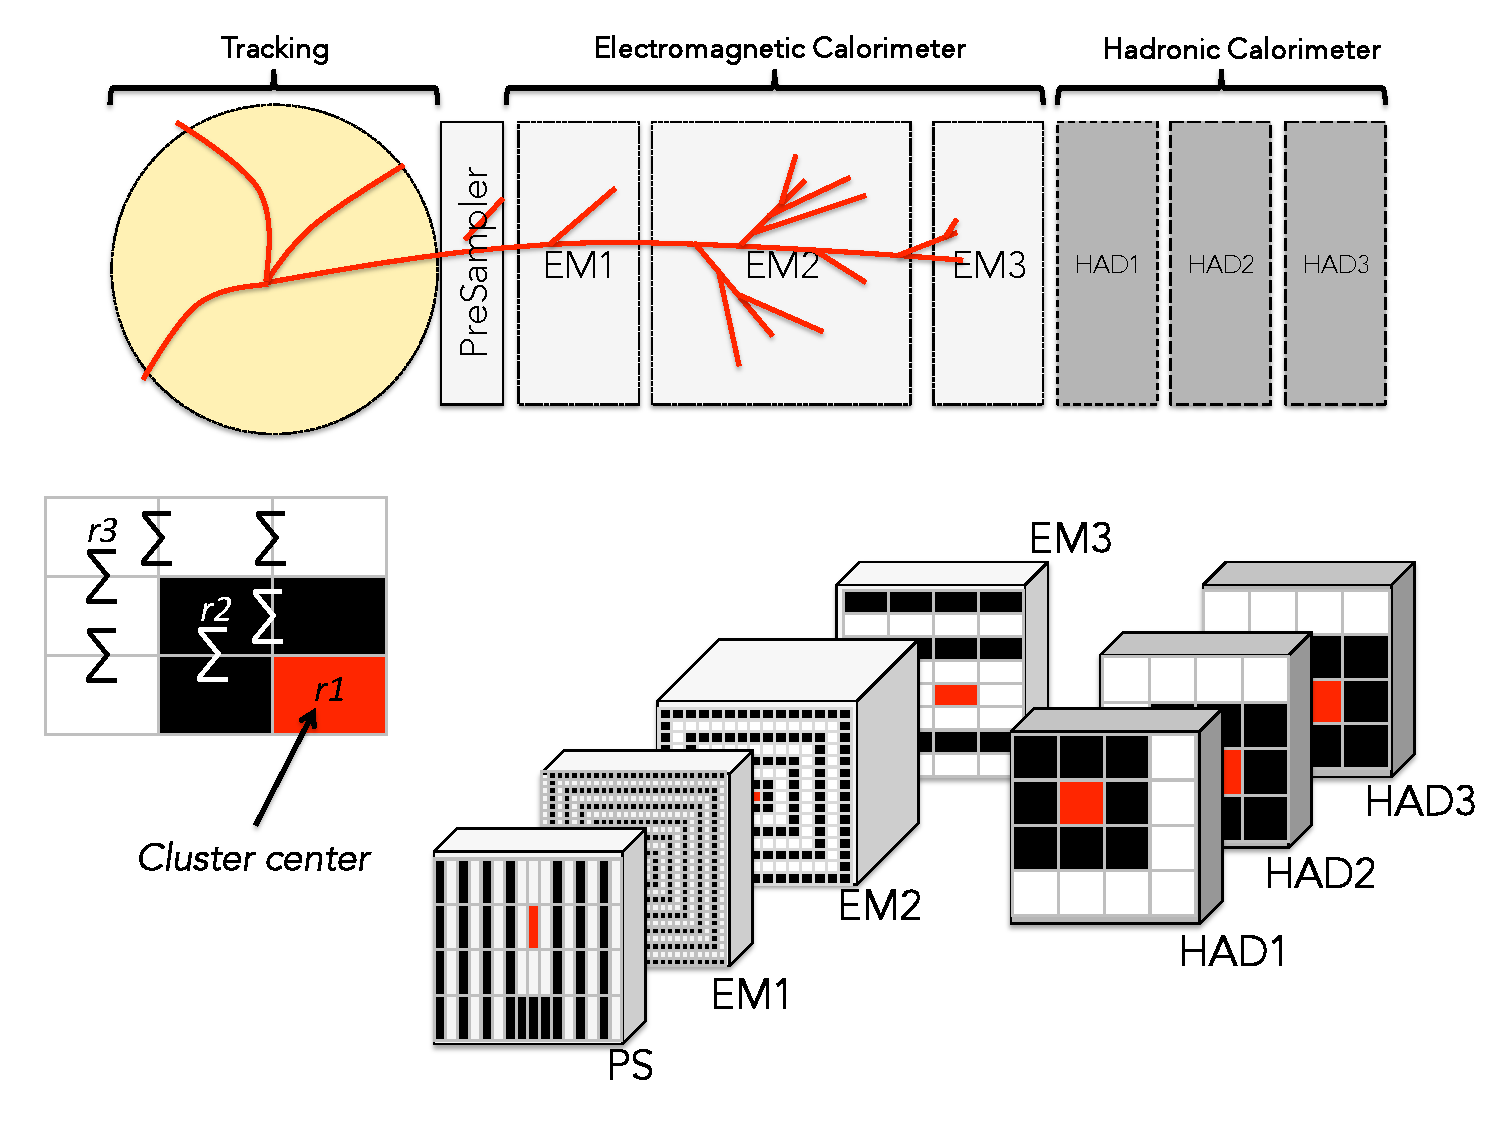
\includegraphics[width=0.8\textwidth]{figures/ringerAlgorithmSketch.pdf}
\caption[Visão simplificada da montagem dos anéis utilizada pelo algoritmo de extração de características.]{Visão simplificada da montagem dos anéis 
utilizada pelo algoritmo de extração de características proposto para cada uma das camadas dos calorímetros.}
\label{fig:ringer_sketch}
\end{figure}

No total, cem anéis são extraídos das sete camadas dos calorímetros. Cada camada tem um número próprio de anéis, de acordo com a sua granularidade. O número de anéis
para cada camada está representado na Tabela~\ref{tab:aneis_por_camada}.


\begin{table}[h]
\centering
\resizebox{\textwidth}{!}{%
\begin{tabular}{cccccccc}
\hline
\hline
\multirow{2}{*}{Camada} & \multicolumn{4}{c}{Calorímetro Eletromagnético} & \multicolumn{3}{c}{Calorímetro Hadrônico} \\ \cline{2-8} 
 & Pre-Sampler & EM.1 & EM.2 & EM.3 & HAD.1 & HAD.2 & HAD.3 \\ \hline
\#anéis & 8 & 64 & 8 & 8 & 4 & 4 & 4 \\ \hline \hline
\end{tabular}%
}
\caption[Número de anéis extraídos em cada camada dos calorímetros]{Número de anéis extraídos para cada uma das camadas dos calorímetros
eletromagnético e hadrônico do \gls{atlas}.}
\label{tab:aneis_por_camada}
\end{table}

\subsection{Algoritmo de Hipótese (HYPO)}

Complementar à nova proposta de extração de características dos calorímetros, também foi desenvolvida uma nova abordagem de
hipótese utilizando uma rede neural artificial  \gls{mlp} como classificador. Esse classificador neural foi implementado na infraestrutura
do \textit{trigger} de forma a ser alimentado pelos anéis do algoritmo de extração. Por definição, a estrutura utilizada é formada 
por cem entradas, uma camada escondida, cujo o número de neurônios é determinado empiricamente pelo método
de treinamento, e apenas um neurônio na camada de saída. A função de ativação de todos os neurônios é a tangente hiperbólica.
A Figura~\ref{fig:topologia_rna} representa uma estrutura genérica de uma rede neural artificial do tipo multi-camada.

\begin{figure}[h!t]
\centering
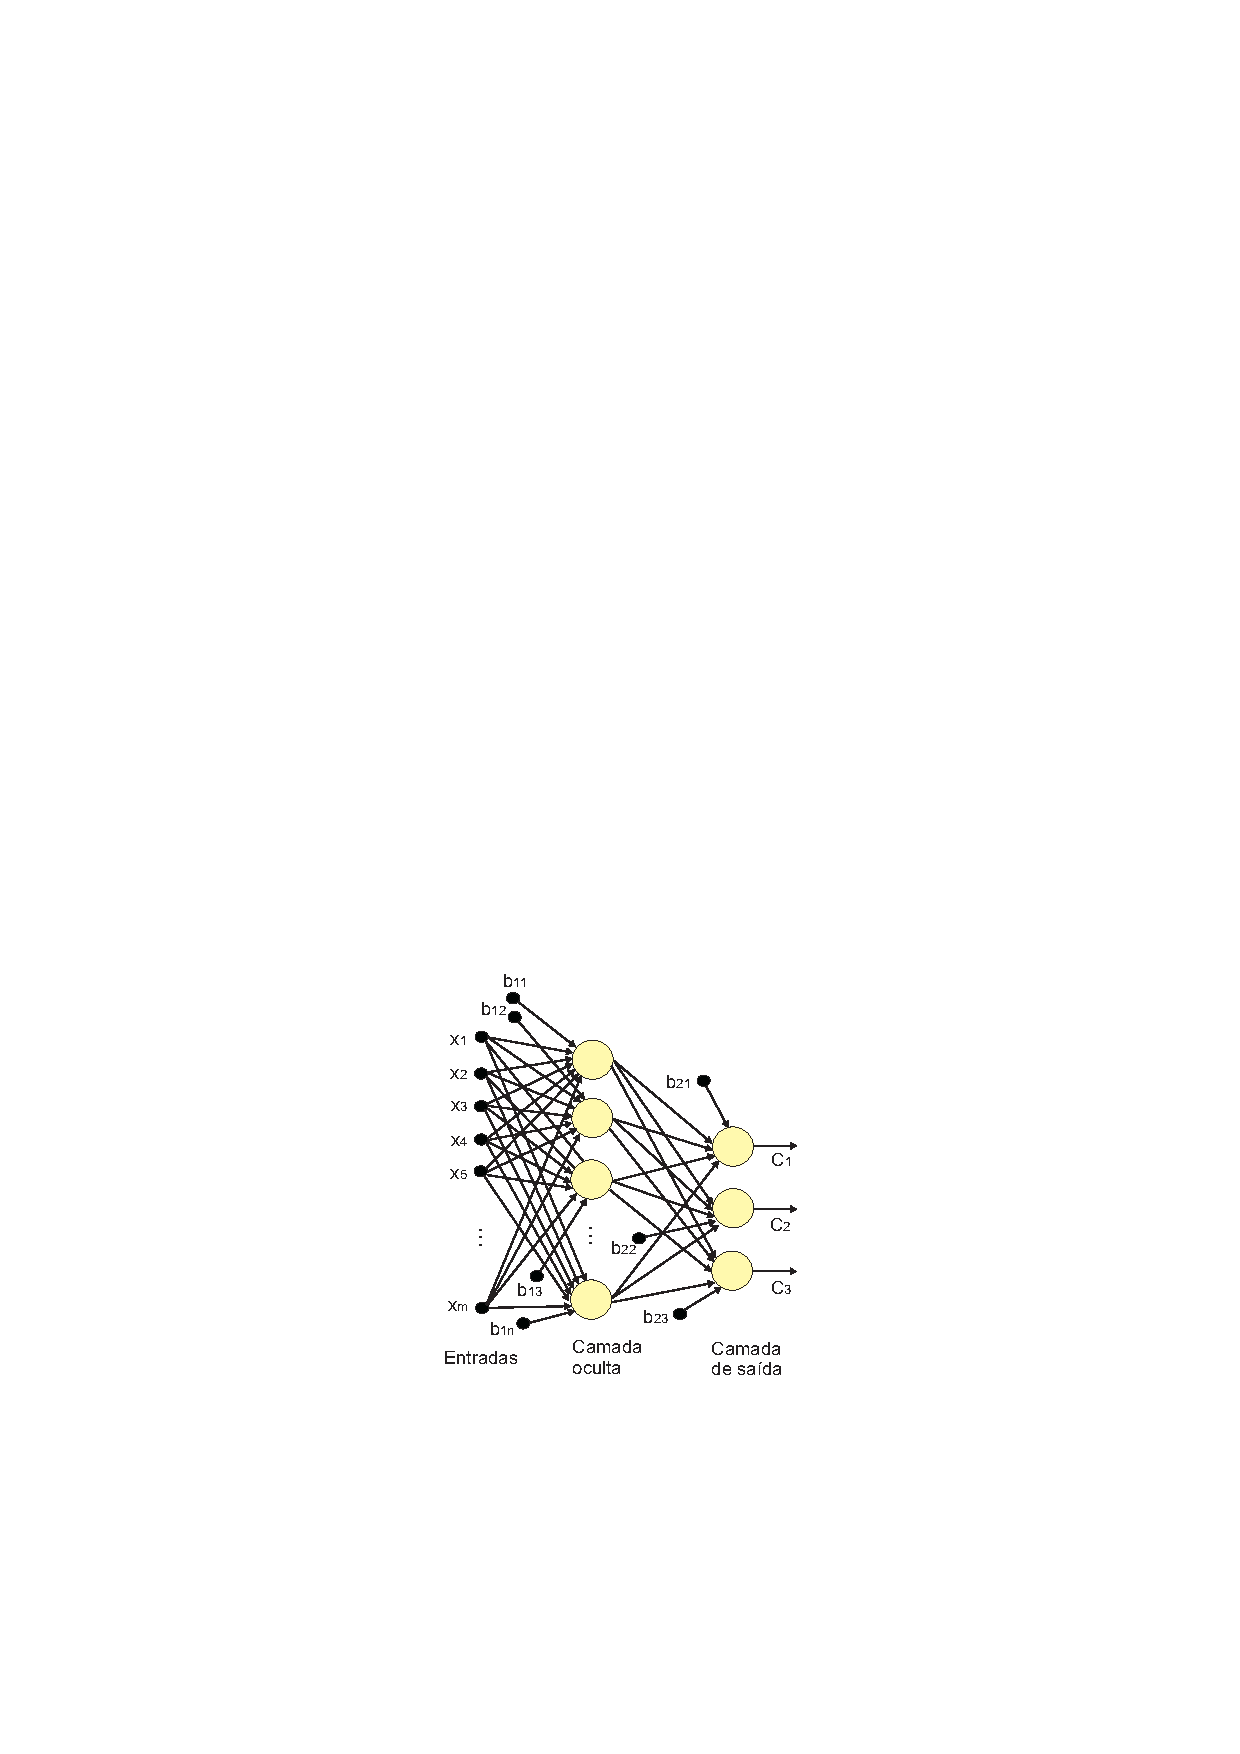
\includegraphics[width=0.4\textwidth]{figures/topologia_rna.pdf}
\caption[Representação da estrutura de uma rede neural do tipo multicamada.]
{Representação da estrutura de uma rede neural do tipo multi-camada, genérica, com apenas uma camada escondida.}
\label{fig:topologia_rna}
\end{figure}

O algoritmo recebe os anéis e realiza um tipo de pré-processamento (o padrão é a normalização de cada anel pela energia total dos anéis)
e repassa essa informação para uma rede neural artificial previamente treinada. Por fim, a saída da rede é comparada com um limiar de corte
que é ajustado dependendo da configuração da \textit{chain} a ser executada pelo \textit{trigger}.

\subsection{Proposta de Assinatura}

Foi selecionada como referência para o treinamento do classificador uma das assinaturas responsáveis pela 
identificação dos elétrons pertencentes ao decaimento $H\rightarrow ZZ\rightarrow 4e$. Assim, o \textit{Neural Ringer}
será comparado com a respectiva etapa de trigger da \textit{chain} de referência escolhida

A otimização do sistema de \textit{trigger} será implementada conforme mostrado na Tabela~\ref{tab:chain_do_ringer}, onde o algoritmo de extração do \textit{ringer},
combinado com a hipótese baseada em um classificado \gls{mlp}, estão localizados na primeira etapa de calorimetria do \textit{trigger} de alto nível.  Assim, uma nova \textit{chain} 
foi criada utilizando o sufixo \textit{ringer} para indicar no \textit{menu} de \textit{trigger} a utilização do algoritmo alternativo \textit{Neural Ringer} na cadeia de filtragem. A assinatura
utilizada como referência também está representada nesta tabela.



\begin{landscape}

% Please add the following required packages to your document preamble:
% \usepackage{multirow}
% \usepackage[table,xcdraw]{xcolor}
% If you use beamer only pass "xcolor=table" option, i.e. \documentclass[xcolor=table]{beamer}
\begin{table}[p]\scriptsize
\centering
\begin{tabular}{ccccccccccc}
\hline
\hline
 & \textbf{L1Calo} & \multicolumn{8}{c}{HLT \textit{\textbf{(High Level Trigger)}}} &  \\ \cline{3-10}
 &  & \multicolumn{4}{c}{{\color[HTML]{333333} \textit{\textbf{Fast}}}} & \multicolumn{4}{c}{{\color[HTML]{000000} \textbf{Precision}}} &  \\ \cline{3-10}
 &  & \multicolumn{2}{c}{{\color[HTML]{333333} \textbf{Calo}}} & \multicolumn{2}{c}{{\color[HTML]{333333} \textbf{Electron}}} & \multicolumn{2}{c}{{\color[HTML]{000000} \textbf{Calo}}} & \multicolumn{2}{c}{{\color[HTML]{000000} \textbf{$e/\gamma$}}} &  \\ \cline{3-10}
\multirow{-4}{*}{\textit{\textbf{Chain}}} &  & {\color[HTML]{FE0000} \textbf{FEX}} & {\color[HTML]{FE0000} \textbf{HYPO}} & {\color[HTML]{333333} FEX} & {\color[HTML]{333333} HYPO} & {\color[HTML]{000000} FEX} & {\color[HTML]{000000} HYPO} & {\color[HTML]{000000} FEX} & {\color[HTML]{000000} HYPO} & \multirow{-4}{*}{\textbf{\begin{tabular}[c]{@{}c@{}}Ajuste \\ do corte\end{tabular}}} \\ \hline
\begin{tabular}[c]{@{}c@{}}e24\_lhmedium\_nod0\_ringer\_iloose\\ (Proposta do Trabalho)\end{tabular} & \begin{tabular}[c]{@{}c@{}}$E_{T} > 20GeV$\\ \\ Isolated\end{tabular} & {\color[HTML]{FE0000} \textbf{Ringer}} & {\color[HTML]{FE0000} \textbf{\begin{tabular}[c]{@{}c@{}}Neural\\ Network\end{tabular}}} & {\color[HTML]{333333} \begin{tabular}[c]{@{}c@{}}FTK\\ +Shower\end{tabular}} & {\color[HTML]{333333} \begin{tabular}[c]{@{}c@{}}T2Calo\\ Combined\end{tabular}} & {\color[HTML]{000000} Shower} & {\color[HTML]{000000} Likelihood} & {\color[HTML]{000000} \begin{tabular}[c]{@{}c@{}}Shower\\ +Tracker\\ +Calibration\end{tabular}} & {\color[HTML]{000000} \begin{tabular}[c]{@{}c@{}}Likelihood\\ Combined\end{tabular}} & medium \\ \hline
\begin{tabular}[c]{@{}c@{}}e24\_lhmedium\_nod0\_iloose\\ (Referência)\end{tabular} & \begin{tabular}[c]{@{}c@{}}$E_{T} > 20GeV$\\ Isolated\end{tabular} & {\color[HTML]{FE0000} \textbf{Shower}} & {\color[HTML]{FE0000} \textbf{T2Calo}} & {\color[HTML]{333333} \begin{tabular}[c]{@{}c@{}}FTK\\ +Shower\end{tabular}} & {\color[HTML]{333333} \begin{tabular}[c]{@{}c@{}}T2Calo\\ Combined\end{tabular}} & {\color[HTML]{000000} Shower} & {\color[HTML]{000000} Likelihood} & {\color[HTML]{000000} \begin{tabular}[c]{@{}c@{}}Shower\\ +Tracker\\ +Calibration\end{tabular}} & {\color[HTML]{000000} \begin{tabular}[c]{@{}c@{}}Likelihood\\ Isolated\end{tabular}} & medium \\
\hline
\hline
\end{tabular}


\caption[Representação do fluxo de algoritmos e cortes realizados para a \textit{chain} do \textit{ringer} e a referência.]
{Representação do fluxo de algoritmos e cortes realizados para a \textit{chain} do \textit{ringer} e a referência. As colunas em vermelho representam as etapas do \textit{trigger} que serão otimizadas.}
\label{tab:chain_do_ringer}
\end{table}

\end{landscape}


\section{Método}

O algoritmo de extração de características do \textit{Neural Ringer} fornece os anéis necessários para a descrição do perfil de deposição de energia da RoI para o \textit{trigger} de alto nível.
O algoritmo de hipótese, baseado numa rede neural, deve operar sobre esses anéis para fornecer a decisão da \textit{chain}. Entretanto, para o treinamento supervisionado
da rede neural, cada RoI deve ser previamente etiquetada de acordo com a sua natureza. No caso de simulações de Monte Carlo, essa informação é feita de acordo 
com a informação da \textit{truth} ou da decisão das análises realizadas pelo \textit{offline}. 

\subsection{Conjunto de Dados}

Os estudos do algoritmo proposto foram realizados utilizando simulações de Monte Carlo de 2014, que contemplam um cenário de operação de energia
envolvida de 13 $TeV$. Nessas condições, a quantidade de empilhamento de eventos é considerável. Na simulação, podem haver, em média, até 20 colisões  
inelásticas. Entretanto, se essas interações ocorrem em uma mesma região do detector, a esse efeito dar-se o nome de empilhamento, a informação sobreposta 
pode impedir a correta identificação das partículas.

Utilizam-se simulações de Monte Carlo para a produção de bósons $Z$ com os algoritmos de hipótese mais atuais e assinaturas \textit{trigger} para a identificação
de elétrons decorrentes do decaimento $Z\rightarrow ee$. Como ruído de fundo do processo de decaimento do bóson $Z$, utilizaram-se simulações de jatos com energia
concentrada em 17 $GeV$, operando sobre as mesmas condições já descritas. As simulações alimentam os emuladores dos sistemas do \gls{atlas} (através do
\textit{framework} do \textit{Athena}), fornecendo uma resposta similar àquela observada experimentalmente.

\subsection{Seleção de Sinais}
\label{sec:selecao_sinais}
As RoI de todos os dados utilizados na simulação de Monte Carlo devem ser classificadas antes da fase de treinamento dos
discriminadores . Assim para a seleção dos elétrons foi utilizada uma abordagem baseada na resposta das análises \textit{offline}. Porém
para o conjunto que irá formar o ruído de fundo, no caso os jatos, será utilizada uma abordagem baseada na natureza da partícula
dada pela própria simulação (\textit{truth}). Os critérios utilizados para a seleção dos eventos para a construção da \textit{chain} proposta são:

\begin{description}
\item[Seleção dos elétrons]: Todas as RoI selecionadas pelo L1 nos dados simulados para o decaimento $Z\rightarrow ee$ são casadas com 
os objetos reconstruídos no ambiente \textit{offline}, através de suas posições $\eta\times\phi$. Posteriormente, um corte de $E_{T}>19GeV$ é aplicado nos \textit{clusters} formados pelo
sistema de calorimetria rápida do \textit{trigger} de alto nível. Por fim, uma RoI é considerada como elétron caso o seu objeto \textit{offline} associado tenha sido aprovado pelo critério \textit{tight} utilizado 
pelo algoritmo de hipótese configurado para esta \textit{chain}.

\item[Seleção dos jatos]: Todas as RoI selecionadas pelo L1 nos dados simulados para os jatos são casadas com seus objetos \textit{truth}, através de suas posições $\eta\times\phi$. 
Posteriormente, um corte de $E_{T}>19GeV$ é aplicado nos \textit{clusters} formados pelo sistema de calorimetria rápida do \textit{trigger} de alto nível. Por fim, uma RoI é considerada 
jato caso sua natureza não seja a de um elétron pela simulação de Monte Carlo.

\end{description}

%A Figura~\ref{fig:perfil_ringer} representa o perfil médio energético, medido em $MeV$, dos anéis para as amostras de elétrons do conjunto de $Z\rightarrow ee$ e de partículas hadrônicas pertencentes 
%ao conjunto de jatos em $E_{T}>17 GeV$. Comparando os dois perfis de energia observa-se que as partículas hadrônicas excitam os anéis mais externos de cada camada além de liberar, em média, 
%mais energia na camada hadrônica. Assim, os jatos possuem um chuveiro mais largo e profundo que as interações dos elétrons no calorímetro. 

%\begin{figure}[h!t]
%\centering
%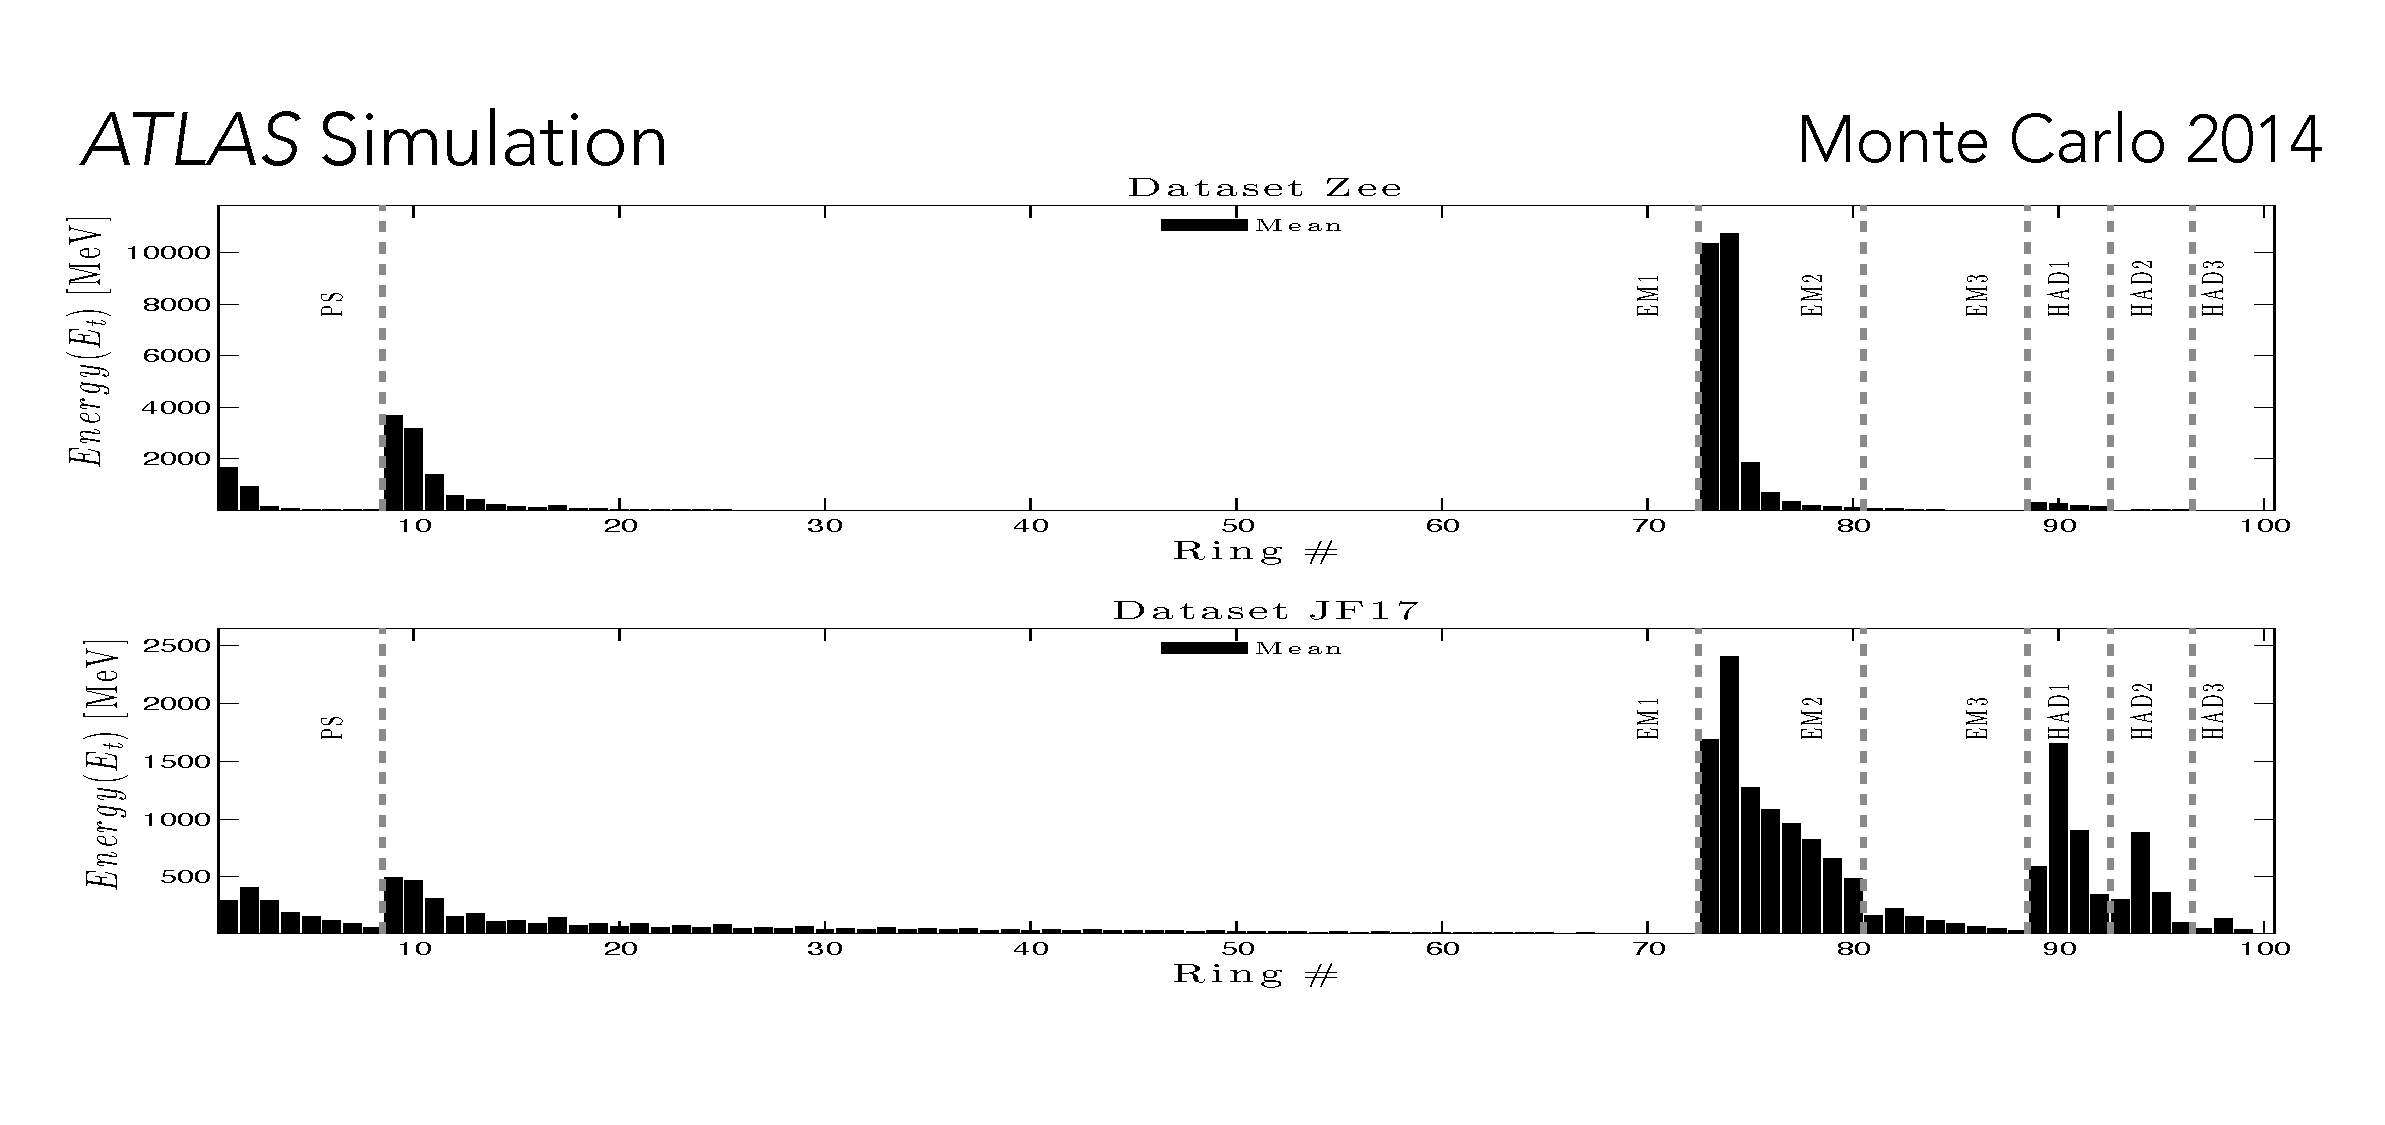
\includegraphics[width=1.0\textwidth]{figures/ringerShape.pdf}
%\caption[Perfil de energia médio para os anéis nas amostras de elétrons e jatos]{Perfis de energia médio, medido em $MeV$, dos anéis para as amostras de elétrons e partículas hadrônicas (jatos).}
%\label{fig:perfil_ringer}
%\end{figure}

\subsection{Estratégia de Trigger}

Os discriminadores neurais são desenvolvidos para a operação no experimento. Assim, a saída da rede neural deve ser comparada com um patamar para a decisão
entre aceitar ou rejeitar a RoI em questão. Esse patamar, porém, pode ser definido por diversas estratégias. Nesse estudo, três estratégias são consideradas.
A primeira considera o ponto de operação do discriminador que consegue a melhor relação entre probabilidade de detecção de elétrons e taxa 
de falso alarme de jatos, segundo o índice SP.

\begin{equation}
SP = \sqrt{ \sqrt{P_{d} \times (1-F_{a})}  \times \frac{(P_{d}+(1-F_{a}))}{2} }
\end{equation}


onde $P_{d}$ é a probabilidade de detecção de elétrons, e $F_{a}$ a taxa de falso alarme do discriminador. A utilização da média geométrica aumenta a sensibilidade em relação as discrepâncias 
entre as duas eficiências. O índice SP pode ser uma alternativa para a escolha de um critério \textit{medium} para o discriminador proposto. As outras duas abordagens consideram a taxa de detecção 
e de falso alarme operadas pelo T2Calo, também, possibilitando a comparação direta entre os dois algoritmos. No entanto, deve-se sempre beneficiar a probabilidade de detecção, já que é esta 
a estratégia comum no sistema \textit{online} de filtragem do ATLAS.


\subsection{Estratégia de Treinamento}


Em todas as abordagens, os conjuntos de RoI de elétrons e jatos foram divididos aleatoriamente em dois conjuntos: o conjunto de treino, utilizado para o ajuste dos 
parâmetros da rede neural com 60\% da base de dados, e o conjunto de teste, utilizado para a avaliação do desempenho de cada discriminador desenvolvido com os 40\% restantes. 
O conjunto de teste também é utilizado como conjunto de validação do treinamento, a fim de evitar o super-treinamento das redes neurais. Normalmente, em experimentos de física de 
partículas, a quantidade produzida de eventos, seja por simulações, seja por aquisições em experimentos reais, é suficiente para a caracterização estatística do processo físico de interesse. 
Dessa forma, não é necessário dividir a base de dados em três conjuntos distintos, como usualmente é feito em projetos de redes neurais.

A arquitetura utilizada foi aquela com melhor desempenho variando-se a quantidade de neurônios na camada escondida da rede neural de 5 até 20.
A rede possui somente uma camada escondida de neurônios e somente um neurônio na camada de saída. Todos os neurônios têm a função tangente hiperbólica 
como função de ativação, onde elétrons são mapeados pelo neurônio de saída em ‘1’ e jatos em ‘-1’.

O algoritmo de treinamento utilizado foi o \textit{resilient backpropagation}  \cite{rprop}, devido à sua rápida convergência.  Os pesos sinápticos da rede são ajustados por batelada, considerando 
o \gls{mse}, como função a ser minimizada. Como a quantidade de RoI de elétrons e de jatos, para alguns casos, é muito diferente, a 
quantidade de RoI utilizadas na batelada é definida pela classe com o menor número de exemplares no treinamento. Posteriormente, para cada época, escolhe-se aleatoriamente 
a mesma quantidade de RoI da classe mais numerosa.

Um método de validação cruzada foi implementado para estimar o impacto da flutuação estatística dos dados utilizados no desempenho dos discriminadores. O método utilizado 
consiste em dividir o conjunto total de dados em $N$ subgrupos, de forma aleatória. Define-se, então, uma quantidade $K$ de sorteios, onde cada sorteio consiste em escolher 
aleatoriamente metade dos $N$ subgrupos para formar o conjunto de treino, e a outra metade para formar o conjunto de teste. A Figura~\ref{fig:crossval} mostra um ilustrativo com a escolha 
de eventos para a validação cruzada.

\begin{figure}[h!t]
\centering
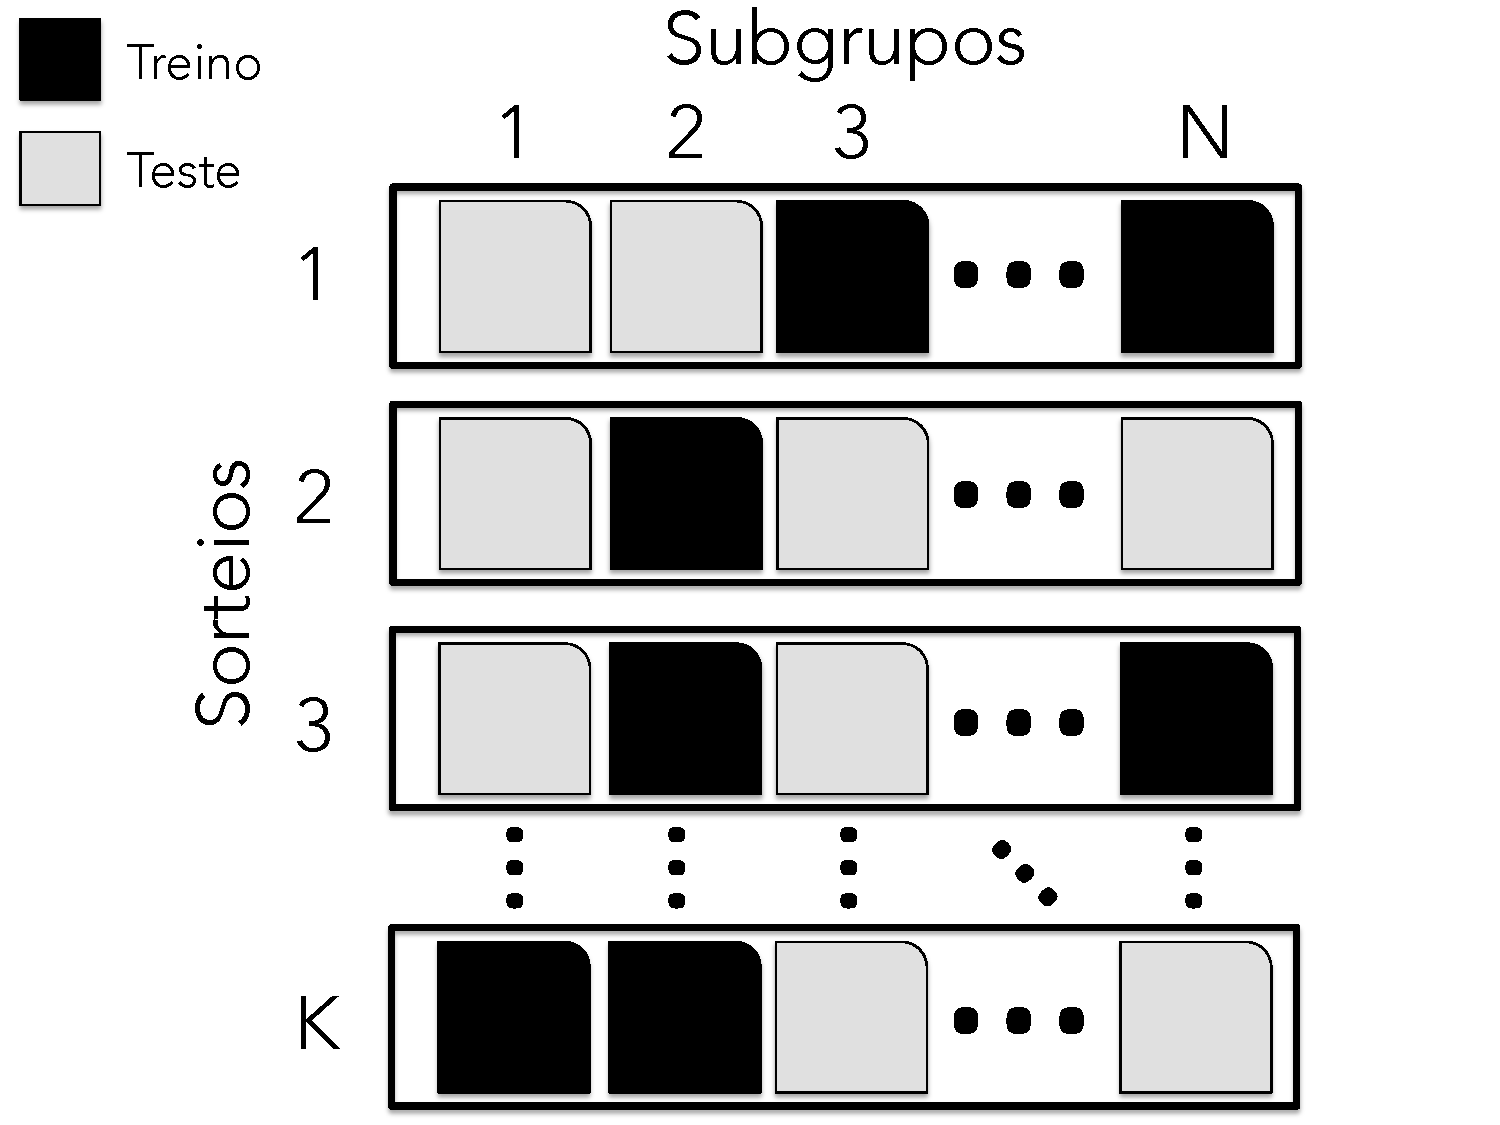
\includegraphics[width=0.4\textwidth]{figures/kfouldFigure.pdf}
\caption[Representação do método de validação cruzada.]{Representação do método de validação cruzada.}
\label{fig:crossval}
\end{figure}

A cada sorteio, escolhe-se aleatoriamente os subgrupos para formar novos conjuntos de treino e teste. Inicializa-se os pesos de 100 discriminadores neurais de forma aleatória, sendo
esta uma técnica de força bruta empregada para escapar de um mínimo local do treinamento. Treina-se os discriminadores para cada sorteio. O discriminador que obtiver o melhor índice SP
avaliado pelo conjunto de teste será arquivado para cada sorteio. Após os $K$ sorteios, 50 sorteios no caso, o desvio padrão dos resultados dos discriminadores arquivados de cada sorteio, em 
conjunto com o valor médio desses resultados, constitui uma boa estimativa do efeito da flutuação estatística dos dados sobre o desempenho da rede neural. No entanto, deve-se escolher 
uma rede dentre as treinadas para diferentes sorteios.

De forma a evitar a polarização do resultado para um determinado  conjunto específico de treino/teste, escolhe-se a rede que obtiver o melhor desempenho utilizando todo o conjunto de dados disponível.
Por fim, antes de alimentar a rede neural, a informação da energia dos anéis deve ser normalizada, de forma a evitar a saturação dos pesos da rede. Diversas normalizações para o 
\textit{Neural Ringer} já foram estudadas~\cite{tese_torres} . Concluiu-se que a normalização mais satisfatória é a divisão do valor de cada anel pela soma do valor de todos os anéis extraídos da RoI.
Embora o \gls{mse} seja escolhido como a função custo, o desempenho da rede é avaliado segundo a sua eficiência na classificação de cada classe. 

A cada época é calculado a probabilidade de detecção e falso alarme, no conjunto de teste, para cada um dos limiares de corte, num intervalo entre [-1,1], testados com a configuração
de pesos atual. Assim, é possível obter o limiar de corte cujo valor de SP foi máximo. De posse desses valores, três critérios de parada sequênciais foram implementados. A parada
por SP prevê a configuração de pesos durante o treinamento cujo SP foi máximo. A parada por detecção salva a configuração de pesos cujo a probabilidade de detecção foi a maior encontrada
durante o treinamento. No caso do falso alarme a ideia é oposta. Ou seja, a melhor configuração será àquela que obtiver o menor falso alarme durante o treinamento.
Caso o índice SP e detecção não aumente e o falso alarme não diminua após um número de épocas, em geral 100, consecutivas, o treinamento é paralisado. Garante-se, também, desta
forma, que não exista  \textit{overfitting} dos resultados. Por fim, três possíveis configurações de pesos referentes a cada um dos critérios discutidos podem ser utilizados posteriormente.



\subsection{\textit{Tag-and-Probe}}

Esse método consiste em utilizar a identificação de duas partículas para a estimação da eficiência de detecção de um determinado algoritmo. É extremamente útil para aplicações em 
dados reais, onde a natureza da partícula observada é desconhecida. A avaliação do desempenho considera um processo físico de interesse, idealmente, aqueles em que o estado 
final de decaimento apresenta duas partículas detectáveis. No caso do bóson de $Z$, por exemplo, o estado final consiste em dois elétrons.

Calcula-se a eficiência a partir da quantidade de objetos \textit{probe} identificados pelo algoritmo avaliado dado que o evento possui um objeto \textit{tag} associado. Ou seja, busca-se 
entre todos os candidatos detectados no evento, aqueles que foram aceitos por um critério extremamente preciso (\textit{tag}), normalmente algum critério \textit{tight}, e possíveis outras considerações. 
Para cada objeto \textit{tag}, busca-se por outros candidatos que, em conjunto com o objeto \textit{tag} selecionado, se aproximem da assinatura do processo físico de interesse (\textit{probe}). 
Normalmente, alguns outros pré-requisitos também são impostos para a seleção desses objetos \textit{probe}. Finalmente, a eficiência é calculada pela razão entre a quantidade de objetos 
\textit{probe} identificados pelo algoritmo avaliado e a quantidade total de objetos \textit{probe} formados.

A imposição de características físicas ao confrontar o par \textit{tag-probe}, de acordo com processo físico de interesse, como, por exemplo, a reconstrução da massa invariante do 
bóson $Z$, aumenta a rejeição do método em relação ao ruído de fundo do experimento. Por isso a sua ampla utilização na colaboração, tanto na avaliação de algoritmos no 
ambiente \textit{online} e \textit{offline}, como na otimização dos cortes utilizados, por exemplo, no algoritmo T2Calo. O método de \textit{tag-and-probe} utilizado nesse estudo utiliza condições e requisitos 
leves para a seleção de cada objeto. Ambos os objetos \textit{tag} e \textit{probe} necessitam de um objeto \textit{offline} associado e que tenha sido aceito pelo critério \textit{tight} de identificação de elétrons. 
Posteriormente, o par formado deve reconstruir a massa invariante do bóson $Z$ no intervalo [80, 100] GeV.  Assim, para o evento ser considerado, um 
dos objetos do \textit{offline} deve ter sido aceito pelo T2Calo (\textit{tag}). A eficiência é calculada, então, como a probabilidade do algoritmo testado aceitar o outro objeto \textit{offline} (\textit{probe}).


\section{Ferramenta de Ajuste dos Pesos da Rede}

Complementar ao problema, o poder computacional para realizar tal experimento utilizando a metodologia de treinamento dos classificadores,
discutida anteriormente, também foi um gargalo que precisou ser otimizado. Assim, optou-se pelo desenvolvimento de um \textit{framework}
que permitisse treinar os inúmeros classificadores de forma totalmente integrada ao ambiente de computação paralela do CERN.
A equação~\ref{eq:total_n_redes} representa o número total de redes neurais que deverão ser treinadas seguindo a metodologia de treinamento, aqui discutida.

\begin{equation}
N_{redes}=N_{sorteios}\times N_{Inits}\times N_{topologias} 
\label{eq:total_n_redes}
\end{equation}

Onde $N_{Sorteios}$ representa o número de sorteios do método de validação cruzada, no caso 50, $N_{Inits}$ o número de inicializações aleatórias
das redes definido como 100 e $N_{Topologias}$ como sendo o número de topologias testadas variando-se o número de neurônios na camada
escondida no intervalo de [5, 20] neurônios, nesse caso 16 topologias avaliadas, totalizando 80 mil redes avaliadas. Dessa forma, o \textit{framework} desenvolvido
precisou conter as seguintes funcionalidades e atender aos seguintes critérios: 

\begin{itemize}

\item Fácil adaptação: O \textit{framework} desenvolvido possui uma interface em \textit{python}, permitindo assim a fácil manutenção e adaptação do código em um
ambiente colaborativo.

\item Ajuste de classificador: o framework possibilita o ajuste de classificadores neurais. O código atual tem como núcleo o \textit{FastNet}, desenvolvido anteriormente pelo 
trabalho~\cite{tese_torres}, em C++. Atualmente o núcleo fornece o treinamento por \gls{rprop} \cite{rprop} e o algoritmo simples de gradiente, ambos
com critérios de parada customizados, no caso da parada pelo índice SP.

\item Adaptação dos dados: O \textit{framework} possibilita a transformação dos dados de saída do \textit{Athena} para o formato \textit{numpy} no \textit{python}. Atualmente isso é feito através da 
entrada de dados formatados, desenvolvido pelo autor deste trabalho em cima do pacote de análise do \textit{trigger} do grupo $e/\gamma$, podendo ser expandido para outros formatos
utilizados pela colaboração

\item Técnica de validação cruzada: Aplicação e medição da técnica de validação cruzada para estimação de flutuações estatísticas.

\item Exportar classificadores: O \textit{framework} deve converter os classificadores a serem utilizados para operação no formato compreendido pelo \textit{Athena}.

%\item Critérios de parada: A aplicação deve conter diferentes critérios de paralisação do treinamento da rede. 

\item Integração com a \textit{grid}: O \textit{framework} deve possibilitar a utilização dos inúmeros computadores pertencentes a \textit{grid} do \gls{cern} para treinar de forma
paralela a grande quantidade de classificadores requeridos.

\end{itemize}

Após a implementação deste \textit{framework} no ambiente do \acrshort{cern}, o tempo de conclusão das análises realizadas para inferir um bom classificador, que 
antes eram de dias, foi reduzido para poucas horas. Permitindo assim, a possibilidade de realizar inúmeros testes e adaptações no método e ou estrutura de
pré-processamento das redes.





